% !TeX spellcheck = en_US
\chapter{Offline Reinforcement Learning}
One major challenge in \ac{RL} is the ability to generalize to different tasks, unlike with supervised learning. \Eg, supervised learning in \ac{CV}, a model can be trained on a large dataset (\eg, ImageNet), then retrained on a smaller dataset to adapt with a specific task. This is possible because it was proven that early layers manage to learn different feature representation What \ac{RL} differs from more conventional supervised learning are large diverse dataset, training procedure, how and when the data is collected, \etc. Offline \ac{RL} is one of proposed solution for \ac{RL} generalization problem. This chapter examines how we can formulate \ac{RL} similar to supervised learning.

\section{Formulation}
Offline \ac{RL} is also known as batch \ac{RL}, fully off-policy \ac{RL}.
\begin{figure}[hbt!]
	\centering
	\begin{subfigure}[b]{0.25\textwidth}
		\centering
		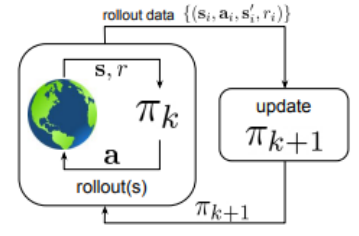
\includegraphics[width=\textwidth]{on-policy-rl.png}
		\caption{On-policy \ac{RL}}
	\end{subfigure}
	\hfill
	\begin{subfigure}[b]{0.25\textwidth}
		\centering
		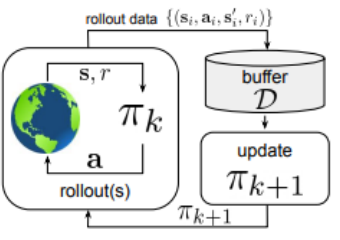
\includegraphics[width=\textwidth]{off-policy-rl.png}
		\caption{Off-policy \ac{RL}}
	\end{subfigure}
	\hfill
	\begin{subfigure}[b]{0.4\textwidth}
		\centering
		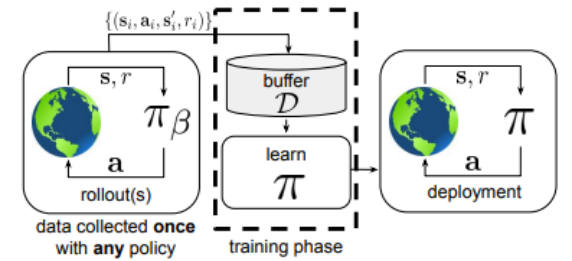
\includegraphics[width=\textwidth]{offline-rl.png}
		\caption{Offline \ac{RL}}
	\end{subfigure}
	\caption{Different settings for \ac{RL}.}
\end{figure}

Formal problem definition: Offline \ac{RL}
\begin{align}
	&\mathcal{D} = \{ (\textbf{s}_i, \textbf{a}_i, \textbf{s}'_i, \textbf{r}_i) \} &&-\text{dataset of transitions}\\
	&\textbf{s} \sim d^{\pi_\beta}(\textbf{s})\\
	&\textbf{a} \sim \pi_\beta(\textbf{a|s}) &&-\text{unknown policy}\\
	&\textbf{s}' \sim p(\textbf{s}'|\textbf{s,a})\\
	&r \leftarrow r(\textbf{s,a})\\
	&\underset{\pi}{\max} \sum_{t=0}^T \mathbb{E}_{\textbf{s}_t \sim d^{\pi_\beta}(\textbf{s}), \textbf{a} \sim \pi(\textbf{a|s})} [\gamma^t r(\textbf{s}_t, \textbf{a}_t)] &&-\text{\ac{RL} objective}
\end{align}

\begin{itemize}
	\item \ac{OPE}: given $\mathcal{D}$, estimate $\displaystyle J(\pi_\beta) = \mathbb{E}_{\pi_\beta} \left[ \sum_{t=1}^T r(\textbf{s}_t, \textbf{a}_t) \right]$
	\item Offline \ac{RL}: given $\mathcal{D}$, learn the \hlb{best possible} policy $\pi_{\theta}$, which might not be the best possible policy for the \ac{MDP}
\end{itemize}

We hope this is possible because: we expect the model can
\begin{itemize}
	\item Find the \textit{"good stuff"} in a dataset full of good and bad behaviors
	\item Generalization: good behavior in one place may suggest good behavior in another place
	\item \textit{"Stitching"}: parts of good behaviors can be recombined \cite{singh2020cog}
\end{itemize}

\section{Challenges}
\begin{itemize}
	\item Little amount of online tuning has significantly more impact than offline training \cite{kalashnikov2018qt}
	\item Distribution shift\\
	\begin{align*}
		&\theta \leftarrow \underset{\theta}{\arg\max} \mathbb{E}_{\textbf{x}\sim p(\textbf{x}), y \sim p(y|\textbf{x})} [(f_\theta(\textbf{x})-y)^2] && -\text{normal regression problem}\\
		&\mathbb{E}_{\textbf{x}'\sim p(\textbf{x})} [(f_\theta(\textbf{x}')-y)^2] &&-\text{is low in expectation}\\
		&\mathbb{E}_{\textbf{x}'\sim \bar{p}(\textbf{x})} [(f_\theta(\textbf{x}')-y)^2] &&-\text{is not, for general $\bar{p}(\textbf{x}) \neq p(\textbf{x})$}\\
		&\mathbb{E}_{\textbf{x}'\sim p(\textbf{x})} [(f_\theta(\textbf{x}')-y)^2] &&-\text{is \hlb{NOT} low if $\textbf{x}' \leftarrow \underset{\textbf{x}}{\arg\max} f_\theta(\textbf{x})$}\\
	\end{align*}
	This is exactly what happens for value-based \ac{RL} approaches, in which we decide the action based on maximizing the value function $\Rightarrow$ Over-estimation of value function \cite{kumar2019stabilizing}
	\item Counterfactual queries: must account for out-of-distribution actions, ideally in a safe way, while still making use of generalization to come up with behaviors that are better than the best thing seen in the data \cite{levine2020offline}
	\item Issues with generalization are not corrected:
	\begin{figure}[hbt!]
		\centering
		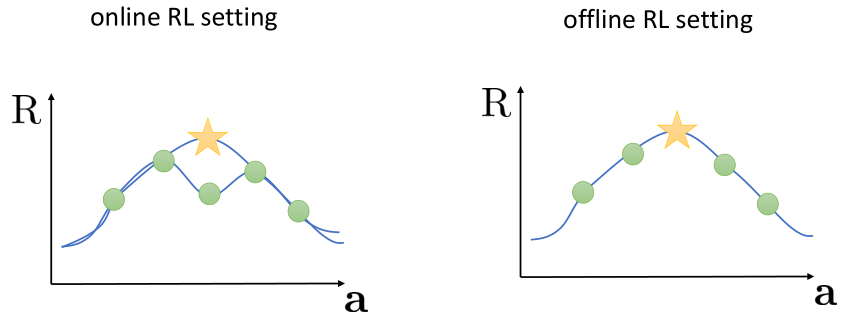
\includegraphics[width=.7\textwidth]{offline-rl-generalization-isse.png}
	\end{figure}	
\end{itemize}

\section{Classic Offline RL}
If you want to use offline \ac{RL} today, you probably would not use approaches in this section.

\subsection{Batch RL via Importance Sampling}
Batch \ac{RL} is just an old name for offline \ac{RL} (around 2000s). Using importance sampling, we can use samples from one policy to learn another one (\secref{sec:off-policy-policy-gradient})

\begin{align*}
	&\underset{\pi}{\max} \sum_{t=0}^T \mathbb{E}_{\textbf{s}_t \sim d^\pi(\textbf{s}), \textbf{a}_t \sim \pi(\textbf{a|s})} [\gamma^t r(\textbf{s}_t, \textbf{a}_t)] \qquad\qquad-\text{\ac{RL} objective}\\
	\nabla_\theta J(\theta) &= \mathbb{E}_{\tau \sim \pi_\theta(\tau)} \left[ \sum_{t=0}^T \nabla_\theta \gamma^t \log \pi(\textbf{a}_t | \textbf{s}_t) \hat{Q}(\textbf{s}_t, \textbf{a}_t) \right] \qquad\qquad-\text{policy gradient}\\
	&\approx \frac{1}{N} \sum_{i=1}^N \sum_{t=0}^T \nabla_\theta \gamma^t \log \pi_\theta(\textbf{a}_{t,i} | \textbf{s}_{t,i}) \hat{Q}(\textbf{s}_{t,i}, \textbf{a}_{t,i}) \qquad\text{requires sampling from $\pi_\theta$}\\
	\nabla_\theta J(\theta) &\approx \frac{1}{N} \sum_{i=1}^N \underbrace{\frac{\pi_\theta(\tau_i)}{\pi_\beta(\tau_i)}}_{\text{importance weight}} \sum_{t=0}^T \nabla_\theta \gamma^t \log \pi_\theta(\textbf{a}_{t,i} | \textbf{s}_{t,i}) \hat{Q}(\textbf{s}_{t,i}, \textbf{a}_{t,i}) \qquad\text{use samples from $\pi_\beta$}\\
	\frac{\pi_\theta(\tau)}{\pi_\beta(\tau)} &= \frac{\cancel{p(\textbf{s}_1)}}{\cancel{p(\textbf{s}_1)}} \frac{\cancel{\prod_t p(\textbf{s}_{t+1} | \textbf{s}_t, \textbf{a}_t)} \pi_\theta(\textbf{a}_t | \textbf{s}_t)}{\cancel{\prod_t p(\textbf{s}_{t+1} | \textbf{s}_t, \textbf{a}_t)} \pi_\beta(\textbf{a}_t | \textbf{s}_t)} \qquad\qquad \text{exponential in $T$}\\
	\hat{Q}(\textbf{s}_{t,i}, \textbf{a}_{t,i})	&= \mathbb{E}_{\pi_\theta} \left[ \sum_{t' = t}^T \gamma^{t'-t} r_{t'} \right] \approx \sum_{t' = t}^T \gamma^{t'-t} r_{t',i} \qquad\qquad\text{single sample estimate}\\
	\Rightarrow \nabla_\theta J(\theta) &\approx \frac{1}{N} \sum_{i=1}^N \sum_{t=0}^T \parunderbrace{\cancel{\left( \prod_{t'=0}^{t-1} \frac{\pi_\theta(\textbf{a}_{t',i} | \textbf{s}_{t',i})}{\pi_\beta(\textbf{a}_{t',i} | \textbf{s}_{t',i})} \right)}}{accounts for difference in \ac{prob} of landing in $\textbf{s}_{t,i}$, we have $\textbf{s}_t \sim d^{\pi_\beta}(\textbf{s}_t)$, but want $\textbf{s}_t \sim d^{\pi_\theta}(\textbf{s}_t)$} \nabla_\theta \gamma^t \log \pi_\theta (\textbf{a}_{t,i} | \textbf{s}_{t,i}) \parunderbrace{\left( \prod_{t'=t}^{T} \frac{\pi_\theta(\textbf{a}_{t',i} | \textbf{s}_{t',i})}{\pi_\beta(\textbf{a}_{t',i} | \textbf{s}_{t',i})} \right)}{accounts for having incorrect $\hat{Q}(\textbf{s}_{t,i}, \textbf{a}_{t,i})$} \hat{Q}(\textbf{s}_{t,i}, \textbf{a}_{t,i})
\end{align*}

\todo{Ignore for now, too many complicated equations}

\subsection{Batch RL via Linear Fitted Value Functions}
Let's go back to the tabular \ac{RL} setting with linear fitted value functions. This method generally doesn't concern with distributional shift, maybe it was not such a big problem with linear models.

High level idea procedure:
\begin{enumerate}
	\item Estimate the reward
	\item Estimate the transitions
	\item Recover the value function
	\item Improve the policy
\end{enumerate}

\begin{align}
	&\Phi &&-\text{feature matrix, size} |S| \times K\\
	&\Phi \textbf{w}_r \approx r &&-\text{reward model}, \textbf{w}_r \in \mathbb{R}^{K\times 1}, r \in \mathbb{R}^{|S| \times 1}\\
	\Rightarrow & \textbf{w}_r = (\Phi^T \Phi)^{-1} \Phi^T \vec{\textbf{r}} &&-\text{least square}
\end{align}

\section{Conservative Q-Learning}
\ac{CQL}

\section{Model-Based Offline RL}
\ac{MOPO}

\section{Summary}
\section{Applications}
\section{Open Questions}

\section{References}
Readings for importance sampling
\begin{itemize}
	\item Classic work on importance sampled policy gradients and return estimation:
	\begin{itemize}
		\item \citeaus{precup2000eligibility}. Eligibility traces for off-policy policy evaluation.
		\item \citeaus{peshkin2002learning}. Learning from scarce experience.
	\end{itemize}
	\item Doubly robust estimators and other improved importance-sampling estimators:
	\begin{itemize}
		\item \citeaus{jiang2016doubly}. Doubly robust off-policy value evaluation for reinforcement learning.
		\item \citeaus{thomas2016data}. Data-efficient off-policy policy evaluation for reinforcement learning.
	\end{itemize}	
	\item Analysis and theory:
	\begin{itemize}
		\item \citeaus{thomas2015high}. High-confidence off-policy evaluation.
	\end{itemize}
	\item Marginalized importance sampling:
	\begin{itemize}
		\item \citeaus{hallak2017consistent}. Consistent on-line off-policy evaluation. 
		\item \citeausm{liu2019off}. Off-policy policy gradient with state distribution correction.
	\end{itemize}
\end{itemize}

Modern offline \ac{RL}:
\begin{itemize}
	\item \citeausm{levine2020offline}. Offline Reinforcement Learning: Tutorial, Review, and Perspectives on Open Problems.
\end{itemize}